\documentclass{beamer}
\usepackage[utf8]{inputenc}
\usepackage{graphicx, epsfig}
\usepackage{amsmath,mathrsfs,amsfonts,amssymb}
\usepackage{floatflt}
\usepackage{epic,ecltree}
\usepackage{mathtext}
\usepackage{fancybox}
\usepackage{fancyhdr}
\usepackage{multirow}
\usepackage{enumerate}
\usepackage{epstopdf}
\usepackage{multicol}
\usepackage{algorithm}
\usepackage[noend]{algorithmic}
\usepackage{tikz}
\usepackage{blindtext}
\usetheme{default}%{Singapore}%{Warsaw}%{Warsaw}%{Darmstadt}
\usecolortheme{default}

\setbeamerfont{title}{size=\Huge}
\setbeamertemplate{footline}[page number]{}

\setbeamertemplate{section in toc}[sections numbered]


\makeatletter
\newcommand\HUGE{\@setfontsize\Huge{35}{40}}
\makeatother    

\setbeamerfont{title}{size=\HUGE}
\beamertemplatenavigationsymbolsempty

% latin bold lower
\newcommand{\ba}{\mathbf{a}} 
\newcommand{\bc}{\mathbf{c}} 
\newcommand{\be}{\mathbf{e}} 
\newcommand{\bh}{\mathbf{h}} 
\newcommand{\bp}{\mathbf{p}} 
\newcommand{\bt}{\mathbf{t}} 
\newcommand{\bs}{\mathbf{s}} 
\newcommand{\bu}{\mathbf{u}} 
\newcommand{\bv}{\mathbf{v}} 
\newcommand{\bw}{\mathbf{w}} 
\newcommand{\bx}{\mathbf{x}} 
\newcommand{\by}{\mathbf{y}} 
\newcommand{\bz}{\mathbf{z}} 

% latin bold upper
\newcommand{\bA}{\mathbf{A}} 
\newcommand{\bB}{\mathbf{B}} 
\newcommand{\bC}{\mathbf{C}} 
\newcommand{\bI}{\mathbf{I}} 
\newcommand{\bJ}{\mathbf{J}} 
\newcommand{\bL}{\mathbf{L}} 
\newcommand{\bM}{\mathbf{M}} 
\newcommand{\bP}{\mathbf{P}}
\newcommand{\bQ}{\mathbf{Q}} 
\newcommand{\bR}{\mathbf{R}} 
\newcommand{\bT}{\mathbf{T}} 
\newcommand{\bU}{\mathbf{U}} 
\newcommand{\bV}{\mathbf{V}} 
\newcommand{\bW}{\mathbf{W}} 
\newcommand{\bX}{\mathbf{X}} 
\newcommand{\bY}{\mathbf{Y}} 
\newcommand{\bZ}{\mathbf{Z}} 

% latin cal upper
\newcommand{\cF}{\mathcal{F}} 
\newcommand{\cG}{\mathcal{G}} 
\newcommand{\cI}{\mathcal{I}} 
\newcommand{\cL}{\mathcal{L}} 
\newcommand{\cM}{\mathcal{M}} 
\newcommand{\cN}{\mathcal{N}} 
\newcommand{\cS}{\mathcal{S}} 
\newcommand{\cT}{\mathcal{T}} 
\newcommand{\cW}{\mathcal{W}} 
\newcommand{\cX}{\mathcal{X}} 
\newcommand{\cZ}{\mathcal{Z}} 

% latin bb upper
\newcommand{\bbE}{\mathbb{E}} 
\newcommand{\bbI}{\mathbb{I}} 
\newcommand{\bbP}{\mathbb{P}} 
\newcommand{\bbR}{\mathbb{R}} 

% greek bold lower
\newcommand{\bepsilon}{\boldsymbol{\epsilon}} 
\newcommand{\btheta}{\boldsymbol{\theta}} 
\newcommand{\blambda}{\boldsymbol{\lambda}} 
\newcommand{\bpi}{\boldsymbol{\pi}} 
\newcommand{\bmu}{\boldsymbol{\mu}} 
\newcommand{\bsigma}{\boldsymbol{\sigma}} 
\newcommand{\bphi}{\boldsymbol{\phi}} 

% greek bold upper
\newcommand{\bSigma}{\boldsymbol{\Sigma}} 

\DeclareMathOperator*{\argmin}{arg\,min}
\DeclareMathOperator*{\argmax}{arg\,max}

\newcommand{\createdgmtitle}[1]{\title[\hbox to 56mm{Deep Generative Models  \hfill\insertframenumber\,/\,\inserttotalframenumber}]
	{\vspace{1cm} \\ Deep Generative Models \\ {\Huge Lecture #1}}
	\author{Roman Isachenko}
	\institute{
	Moscow Institute of Physics and Technology
	} 
	\date{2023, Autumn}
}

\usepackage{tikz}
\usetikzlibrary{arrows,shapes,positioning,shadows,trees}

\newcommand\myfootnote[1]{%
  \tikz[remember picture,overlay]
  \draw (current page.south west) +(1in + \oddsidemargin,0.5em)
  node[anchor=south west,inner sep=0pt]{\parbox{\textwidth}{%
      \rlap{\rule{10em}{0.4pt}}\raggedright\scriptsize \textit{#1}}};}

\newcommand\myfootnotewithlink[2]{%
  \tikz[remember picture,overlay]
  \draw (current page.south west) +(1in + \oddsidemargin,0.5em)
  node[anchor=south west,inner sep=0pt]{\parbox{\textwidth}{%
      \rlap{\rule{10em}{0.4pt}}\raggedright\scriptsize\href{#1}{\textit{#2}}}};}
      
\AtBeginSection[]
      {
      	\begin{frame}{Outline}
      		\tableofcontents[currentsection]
      	\end{frame}
      }
      \AtBeginSubsection[]{
      	\begin{frame}{Outline}
      		\tableofcontents[currentsection,currentsubsection]
      	\end{frame}
}
\createdgmtitle{11}

\usepackage{tikz}

\usetikzlibrary{arrows,shapes,positioning,shadows,trees}
%--------------------------------------------------------------------------------
\begin{document}
%--------------------------------------------------------------------------------
\begin{frame}[noframenumbering,plain]
%\thispagestyle{empty}
\titlepage
\end{frame}
%=======
\begin{frame}{Recap of previous lecture}
	Consider Ordinary Differential Equation    
	\begin{align*}
	    \frac{d \bz(t)}{dt} &= f_{\btheta}(\bz(t), t); \quad \text{with initial condition }\bz(t_0) = \bz_0. \\
	    \bz(t_1) &= \int^{t_1}_{t_0} f_{\btheta}(\bz(t), t) d t  + \bz_0 = \text{ODESolve}(\bz(t_0), f_{\btheta}, t_0,t_1).
	\end{align*}
	\vspace{-0.4cm}
	\begin{block}{Euler update step}
		\vspace{-0.6cm}
		\[
			\frac{\bz(t + \Delta t) - \bz(t)}{\Delta t} = f_{\btheta}(\bz(t), t) \,\, \Rightarrow \,\, \bz(t + \Delta t) = \bz(t) + \Delta t \cdot f_{\btheta}(\bz(t), t)
		\]
		\vspace{-0.7cm}
	\end{block}
	\begin{block}{Residual block}
		\vspace{-0.4cm}
		\[
			\bz_{t + 1} = \bz_t + f_{\btheta}(\bz_t)
		\]
		It is equivalent to Euler update step for solving ODE with $\Delta t = 1$!
	\end{block}
	In the limit of adding more layers and taking smaller steps we get: 
	\[
	    \frac{d \bz(t)}{dt} = f_{\btheta}(\bz(t), t); \quad \bz(t_0) = \bx; \quad \bz(t_1) = \by.
	\]

	\myfootnotewithlink{https://arxiv.org/abs/1806.07366}{Chen R. T. Q. et al. Neural Ordinary Differential Equations, 2018}   
\end{frame}
%=======
\begin{frame}{Recap of previous lecture}
	\begin{block}{Forward pass (loss function)}
		\vspace{-0.8cm}
		\begin{align*}
			L(\by) = L(\bz(t_1)) &= L\left( \bz(t_0) + \int_{t_0}^{t_1} f_{\btheta}(\bz(t), t) dt \right) \\ &= L\bigl(\text{ODESolve}(\bz(t_0), f_{\btheta}, t_0,t_1) \bigr)
		\end{align*}
	\vspace{-0.5cm}
	\end{block}
	\textbf{Note:} ODESolve could be any method (Euler step, Runge-Kutta methods).
	\begin{block}{Backward pass (gradients computation)}
		For fitting parameters we need gradients:
		\[
			\ba_{\bz}(t) = \frac{\partial L(\by)}{\partial \bz(t)}; \quad \ba_{\btheta}(t) = \frac{\partial L(\by)}{\partial \btheta(t)}.
		\]
		In theory of optimal control these functions called \textbf{adjoint} functions. 
		They show how the gradient of the loss depends on the hidden state~$\bz(t)$ and parameters $\btheta$.
	\end{block}

	\myfootnotewithlink{https://arxiv.org/abs/1806.07366}{Chen R. T. Q. et al. Neural Ordinary Differential Equations, 2018}     
\end{frame}
%=======
\begin{frame}{Recap of previous lecture}
		\vspace{-0.3cm}
		\[
		\ba_{\bz}(t) = \frac{\partial L(\by)}{\partial \bz(t)}; \quad \ba_{\btheta}(t) = \frac{\partial L(\by)}{\partial \btheta(t)} \text{-- adjoint functions}.
		\]
		\vspace{-0.3cm}
	\begin{block}{Theorem (Pontryagin)}
	\vspace{-0.6cm}
	\[
		\frac{d \ba_{\bz}(t)}{dt} = - \ba_{\bz}(t)^T \cdot \frac{\partial f_{\btheta}(\bz(t), t)}{\partial \bz}; \quad \frac{d \ba_{\btheta}(t)}{dt} = - \ba_{\bz}(t)^T \cdot \frac{\partial f_{\btheta}(\bz(t), t)}{\partial \btheta}.
	\]
	\vspace{-0.6cm}
	\end{block}
	\begin{block}{Forward pass}
		\vspace{-0.5cm}
		\[
		\bz(t_1) = \int^{t_1}_{t_0} f_{\btheta}(\bz(t), t) d t  + \bz_0 \quad \Rightarrow \quad \text{ODE Solver}
		\]
		\vspace{-0.6cm}
	\end{block}
	\begin{block}{Backward pass}
		\vspace{-0.6cm}
		\begin{equation*}
			\left.
			{\footnotesize 
				\begin{aligned}
					\frac{\partial L}{\partial \btheta(t_0)} &= \ba_{\btheta}(t_0) =  - \int_{t_1}^{t_0} \ba_{\bz}(t)^T \frac{\partial f_{\btheta}(\bz(t), t)}{\partial \btheta(t)} dt + 0 \\
					\frac{\partial L}{\partial \bz(t_0)} &= \ba_{\bz}(t_0) =  - \int_{t_1}^{t_0} \ba_{\bz}(t)^T \frac{\partial f_{\btheta}(\bz(t), t)}{\partial \bz(t)} dt + \frac{\partial L}{\partial \bz(t_1)} \\
					\bz(t_0) &= - \int^{t_0}_{t_1} f_{\btheta}(\bz(t), t) d t  + \bz_1.
				\end{aligned}
			}
			\right\rbrace
			\Rightarrow
			\text{ODE Solver}
		\end{equation*}
		\vspace{-0.4cm} 
	\end{block}
	\myfootnotewithlink{https://arxiv.org/abs/1806.07366}{Chen R. T. Q. et al. Neural Ordinary Differential Equations, 2018}   
\end{frame}
%=======
\begin{frame}{Recap of previous lecture}
	\begin{block}{Continuous-in-time normalizing flows}
		\vspace{-0.5cm}
		\[
			\frac{d\bz(t)}{dt} = f_{\btheta}(\bz(t), t); \quad \frac{d \log p(\bz(t), t)}{d t} = - \text{tr} \left( \frac{\partial f_{\btheta}(\bz(t), t)}{\partial \bz(t)} \right).
		\]
		\vspace{-0.7cm}
	\end{block}
	\begin{block}{Theorem (Picard)}
		If $f$ is uniformly Lipschitz continuous in $\bz$ and continuous in $t$, then the ODE has a \textbf{unique} solution.
	\end{block}
	\begin{block}{Forward transform + log-density}
		\vspace{-0.4cm}
		\[
			\begin{bmatrix}
				\bx \\
				\log p(\bx | \btheta)
			\end{bmatrix}
			= 
			\begin{bmatrix}
				\bz \\
				\log p(\bz)
			\end{bmatrix} + 
			\int_{t_0}^{t_1} 
			\begin{bmatrix}
				f_{\btheta}(\bz(t), t) \\
				- \text{tr} \left( \frac{\partial f_{\btheta}(\bz(t), t)}{\partial \bz(t)} \right) 
			\end{bmatrix} dt.
		\]
		\vspace{-0.4cm}
	\end{block}	
	\begin{block}{Hutchinson's trace estimator}
		\vspace{-0.3cm}
		\[
		   \log p(\bz(t_1)) = \log p(\bz(t_0)) - \mathbb{E}_{p(\bepsilon)} \int_{t_0}^{t_1} \left[ {\color{violet}\bepsilon^T \frac{\partial f}{\partial \bz}} \bepsilon \right] dt.
		\]
	\end{block}
	\myfootnotewithlink{https://arxiv.org/abs/1810.01367}{Grathwohl W. et al. FFJORD: Free-form Continuous Dynamics for Scalable Reversible Generative Models, 2018} 
\end{frame}
%=======
\begin{frame}{Outline}
	\tableofcontents
\end{frame}
%=======
\begin{frame}{Generative models zoo}
	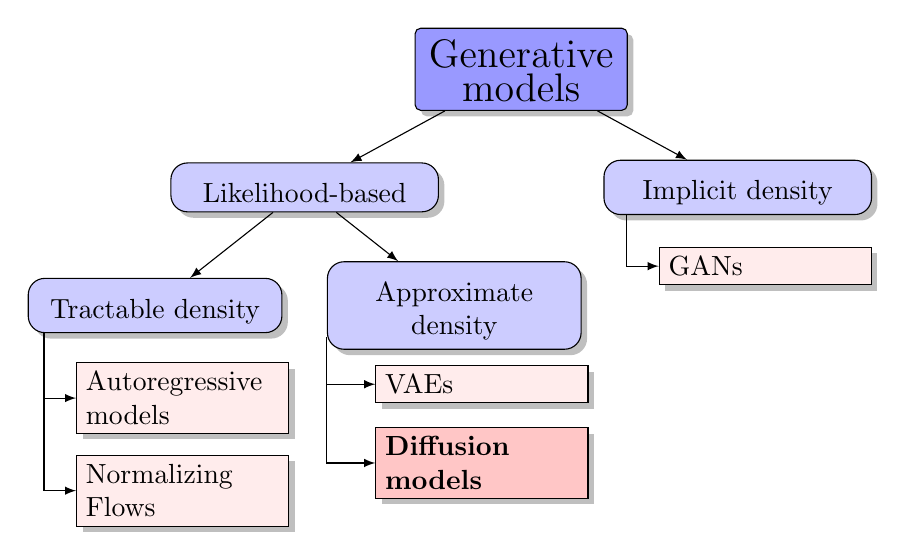
\begin{tikzpicture}[
		basic/.style  = {draw, text width=2cm, drop shadow, rectangle},
		root/.style   = {basic, rounded corners=2pt, thin, text height=1.1em, text width=7em, align=center, fill=blue!40},
		level 1/.style={sibling distance=55mm},
		level 2/.style = {basic, rounded corners=6pt, thin, align=center, fill=blue!20, text height=1.1em, text width=9em, sibling distance=38mm},
		level 3/.style = {basic, rounded corners=6pt, thin,align=center, fill=blue!20, text width=8.5em},
		level 4/.style = {basic, thin, align=left, fill=pink!30, text width=7em},
		level 5/.style = {basic, thin, align=left, fill=pink!90, text width=7em},
		edge from parent/.style={->,draw},
		>=latex]
		
		% root of the the initial tree, level 1
		\node[root] {\Large Generative models}
		% The first level, as children of the initial tree
		child {node[level 2] (c1) {Likelihood-based}
			child {node[level 3] (c11) {Tractable density}}
			child {node[level 3] (c12) {Approximate density}}
		}
		child {node[level 2] (c2) {Implicit density}};
		
		% The second level, relatively positioned nodes
		\begin{scope}[every node/.style={level 4}]
			\node [below of = c11, yshift=-5pt, xshift=10pt] (c111) {Autoregressive models};
			\node [below of = c111, yshift=-5pt] (c112) {Normalizing Flows};
			\node [below of = c12, xshift=10pt] (c121) {VAEs};
			
			\node [below of = c2, xshift=10pt] (c21) {GANs};
		\end{scope}
		
		% The second level, relatively positioned nodes
		\begin{scope}[every node/.style={level 5}]
			\node [below of = c121] (c122) {\textbf{Diffusion \\ models}};
		\end{scope}
		
		% lines from each level 1 node to every one of its "children"
		\foreach \value in {1,2}
		\draw[->] (c11.194) |- (c11\value.west);
		
		\foreach \value in {1,2}
		\draw[->] (c12.194) |- (c12\value.west);
		
		\draw[->] (c2.194) |- (c21.west);
		
	\end{tikzpicture}
\end{frame}
%=======
\section{Gaussian diffusion process}
%=======
\subsection{Forward gaussian diffusion process}
%=======
\begin{frame}{Forward gaussian diffusion process}
	Let $\bx_0 = \bx \sim \pi(\bx)$, $\beta_t \in (0, 1)$. Define the Markov chain
	\[
		\bx_t = \sqrt{1 - \beta_t} \cdot \bx_{t - 1} + \sqrt{\beta_t} \cdot \bepsilon, \quad \text{where }\bepsilon \sim \cN(0, \bI);
	\]
	\[
		q(\bx_t | \bx_{t-1}) = \cN(\bx_t | \sqrt{1 - \beta_t} \cdot \bx_{t-1}, \beta_t \cdot \bI).
	\]
	\vspace{-0.5cm}
	\begin{block}{Statement 1}
		Let denote $\alpha_t = 1 - \beta_t$ and $\bar{\alpha}_t = \prod_{s=1}^t \alpha_s$. Then
		\vspace{-0.2cm}
		\begin{multline*}
			\bx_t = \sqrt{\alpha_t} {\color{teal}\bx_{t-1}} + \sqrt{1 - \alpha_t} \boldsymbol{\epsilon}_t = \\
			= \sqrt{\alpha_t} ({\color{teal} \sqrt{\alpha_{t-1}} \bx_{t-2} + \sqrt{1 - \alpha_{t-1}} \boldsymbol{\epsilon}_{t-1}}) + \sqrt{1 - \alpha_t} \boldsymbol{\epsilon}_t = \\
			= \sqrt{\alpha_t \alpha_{t-1}} \bx_{t-2} + ( \sqrt{\alpha_t (1 - \alpha_{t-1})}  \boldsymbol{\epsilon}_{t-1} + \sqrt{1 - \alpha_t} \boldsymbol{\epsilon}_t) = \\
			= \sqrt{\bar{\alpha}_t} \cdot \bx_{0} + \sqrt{1 - \bar{\alpha}_t} \cdot \bepsilon, \quad \text{where } \bepsilon \sim \cN(0, \bI).
		\end{multline*}
		\vspace{-0.4cm}
		\[
			q(\bx_t | \bx_0) = \cN(\bx_t | \sqrt{\bar{\alpha}_t} \cdot \bx_0, (1 - \bar{\alpha}_t) \cdot \bI).
		\]
		We could sample from any timestamp using only $\bx_0$!
	\end{block}
	\myfootnotewithlink{http://proceedings.mlr.press/v37/sohl-dickstein15.pdf}{Sohl-Dickstein J. Deep Unsupervised Learning using Nonequilibrium Thermodynamics, 2015}
 \end{frame}
%=======
\begin{frame}{Forward gaussian diffusion process}
	\vspace{-0.5cm}
	\begin{align*}
		q(\bx_t | \bx_{t-1}) &= \cN(\bx_t | \sqrt{1 - \beta_t} \cdot \bx_{t-1}, \beta_t \cdot \bI); \\
		q(\bx_t | \bx_0) &= \cN(\bx_t | \sqrt{\bar{\alpha}_t} \cdot \bx_0, (1 - \bar{\alpha}_t) \cdot \bI).
	\end{align*}
	At each step we
	\begin{itemize}
		\item scale magnitude of the signal at rate $\sqrt{1 - \beta_t}$;
		\item add noise with variance $\beta_t$.
	\end{itemize}
	\begin{block}{Statement 2}
		Applying the Markov chain to samples from any $\pi(\bx)$ we will get $\bx_{\infty} \sim p_{\infty}(\bx) = \cN(0, 1)$. Here $p_{\infty}(\bx)$ is a \textbf{stationary} and \textbf{limiting} distribution:
		\vspace{-0.2cm}
		\[
			p_{\infty}(\bx) = \int q(\bx | \bx') p_{\infty}(\bx') d \bx'. 
		\]
		\[
			p_{\infty}(\bx) = \int q(\bx_{\infty} | \bx_0) \pi(\bx_0) d\bx_0 \approx \cN(0, \bI) \int \pi(\bx_0) d\bx_0 = \cN(0, \bI)
		\]
		\vspace{-0.8cm}
	\end{block}
	\myfootnotewithlink{http://proceedings.mlr.press/v37/sohl-dickstein15.pdf}{Sohl-Dickstein J. Deep Unsupervised Learning using Nonequilibrium Thermodynamics, 2015}
 \end{frame}
%=======
\begin{frame}{Forward gaussian diffusion process}
	\textbf{Diffusion} refers to the flow of particles from high-density regions towards low-density regions.
	\vspace{-0.2cm}
	\begin{figure}
		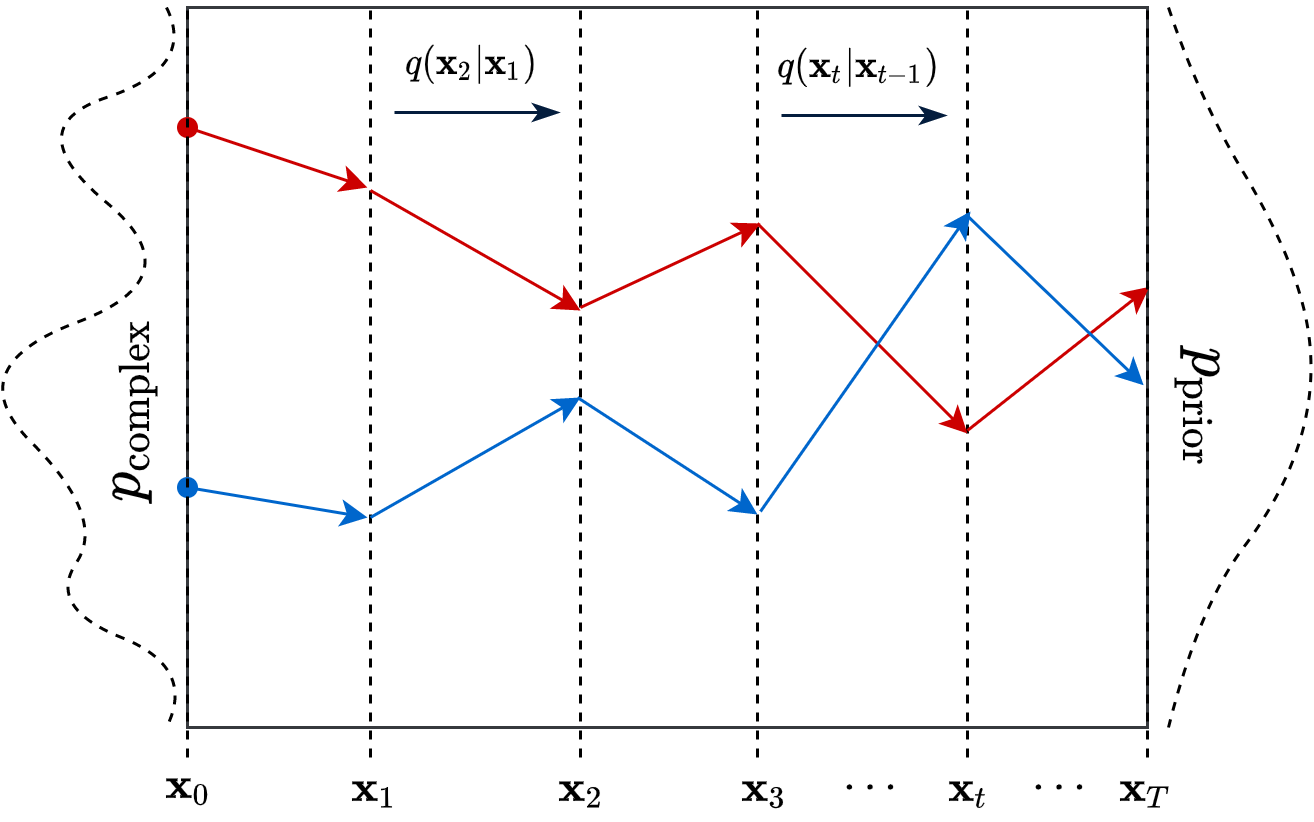
\includegraphics[width=0.5\linewidth]{figs/diffusion_over_time}
	\end{figure}
	\vspace{-0.6cm}
	\begin{enumerate}
		\item $\bx_0 = \bx \sim \pi(\bx)$;
		\item $\bx_t = \sqrt{1 - \beta} \cdot \bx_{t - 1} + \sqrt{\beta} \cdot \bepsilon$, where $\bepsilon \sim \cN(0, 1)$, $t \geq 1$;
		\item $\bx_T \sim p_{\infty}(\bx) = \cN(0, 1)$, where $T >> 1$.
	\end{enumerate}
	If we are able to invert this process, we will get the way to sample $\bx \sim \pi(\bx)$ using noise samples $p_{\infty}(\bx) = \cN(0, 1)$. \\ 
	Now our goal is to revert this process.
	\myfootnotewithlink{https://ayandas.me/blog-tut/2021/12/04/diffusion-prob-models.html}{Das A. An introduction to Diffusion Probabilistic Models, blog post, 2021}
\end{frame}
%=======
\subsection{Reverse gaussian diffusion process}
%=======
\begin{frame}{Reverse gaussian diffusion process}
	\begin{figure}
		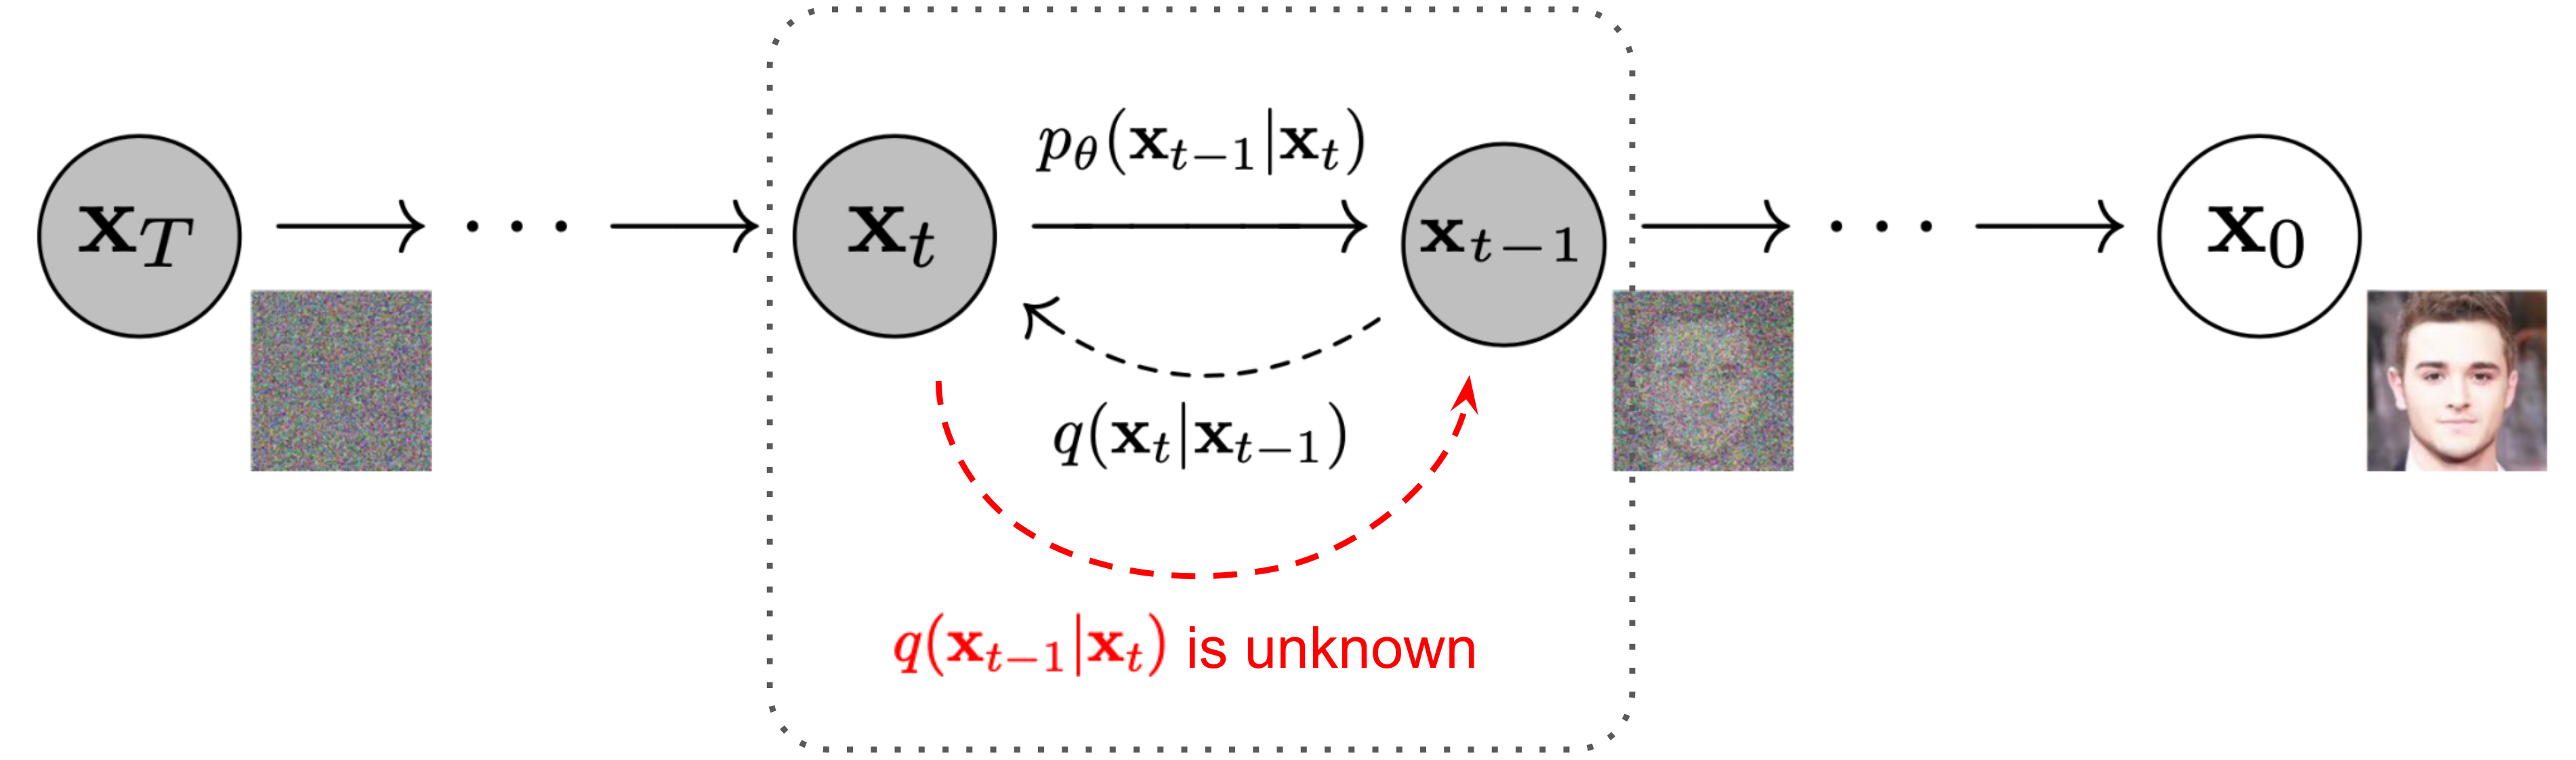
\includegraphics[width=0.8\linewidth]{figs/DDPM}
	\end{figure}
	\vspace{-0.5cm}
	\begin{block}{Forward process}
		\vspace{-0.3cm}
		\[
			q(\bx_t | \bx_{t-1}) = \cN(\bx_t | \sqrt{1 - \beta_t} \cdot \bx_{t-1}, \beta_t \cdot \bI).
		\]
		\vspace{-0.5cm}
	\end{block}
	\begin{block}{Reverse process}
		\vspace{-0.3cm}
		\[
			q(\bx_{t-1}|\bx_{t}) = \frac{q(\bx_{t}|\bx_{t-1}) {\color{violet}q(\bx_{t-1})}}{{\color{violet}q(\bx_{t})}} \approx p(\bx_{t - 1} | \bx_t, \btheta)
		\]
		\vspace{-0.3cm}
		\begin{itemize}
			\item ${\color{violet}q(\bx_{t-1})}$, ${\color{violet}q(\bx_{t})}$ are intractable.
			\item If $\beta_t$ is small enough, $q(\bx_{t-1}|\bx_{t})$ will be Gaussian (Feller, 1949).
		\end{itemize}
	\end{block}
	\myfootnotewithlink{}{Feller W. On the theory of stochastic processes, with particular reference to applications, 1949}
	\end{frame}
%=======
\begin{frame}{Reverse gaussian diffusion process}
		\vspace{-0.4cm}
		\begin{align*}
			q(\bx_{t-1}|\bx_{t}) &= \frac{q(\bx_{t}|\bx_{t-1}) {\color{violet}q(\bx_{t-1})}}{{\color{violet}q(\bx_{t})}} \\
			q(\bx_{t-1}|\bx_{t}, {\color{olive}\bx_0}) &= \frac{q(\bx_{t}|\bx_{t-1}, {\color{olive}\bx_0}) q(\bx_{t-1} | {\color{olive}\bx_0}) }{q(\bx_{t}| {\color{olive}\bx_0})} = \cN(\tilde{\bmu}_t(\bx_t, \bx_0), \tilde{\beta}_t \bI)
		\end{align*}
		\vspace{-0.2cm}
		\begin{itemize}
			\item ${\color{violet}q(\bx_{t-1})}$, ${\color{violet}q(\bx_{t})}$ are intractable.
			\item If $\beta_t$ is small enough, $q(\bx_{t-1}|\bx_{t})$ will be Gaussian (Feller, 1949).
		\end{itemize}
	\vspace{-0.2cm}
	\begin{figure}
		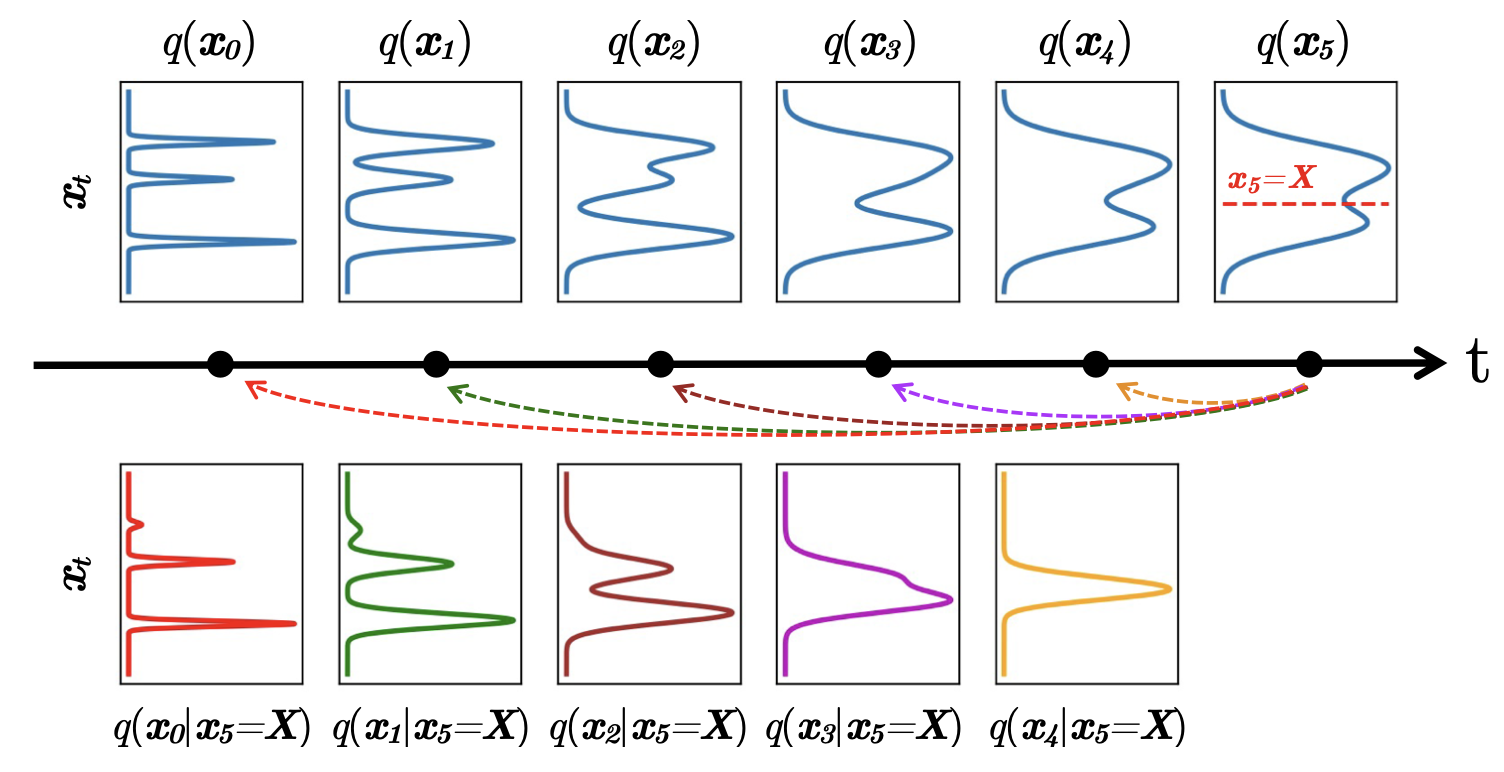
\includegraphics[width=0.7\linewidth]{figs/inverse_distr_1d}
	\end{figure}
	\myfootnotewithlink{https://arxiv.org/abs/2112.07804}{Xiao Z., Kreis K., Vahdat A. Tackling the generative learning trilemma with denoising diffusion GANs, 2021}
	\end{frame} 
%=======
\begin{frame}{Reverse gaussian diffusion process}
	\vspace{-0.3cm} 
	\begin{figure}
		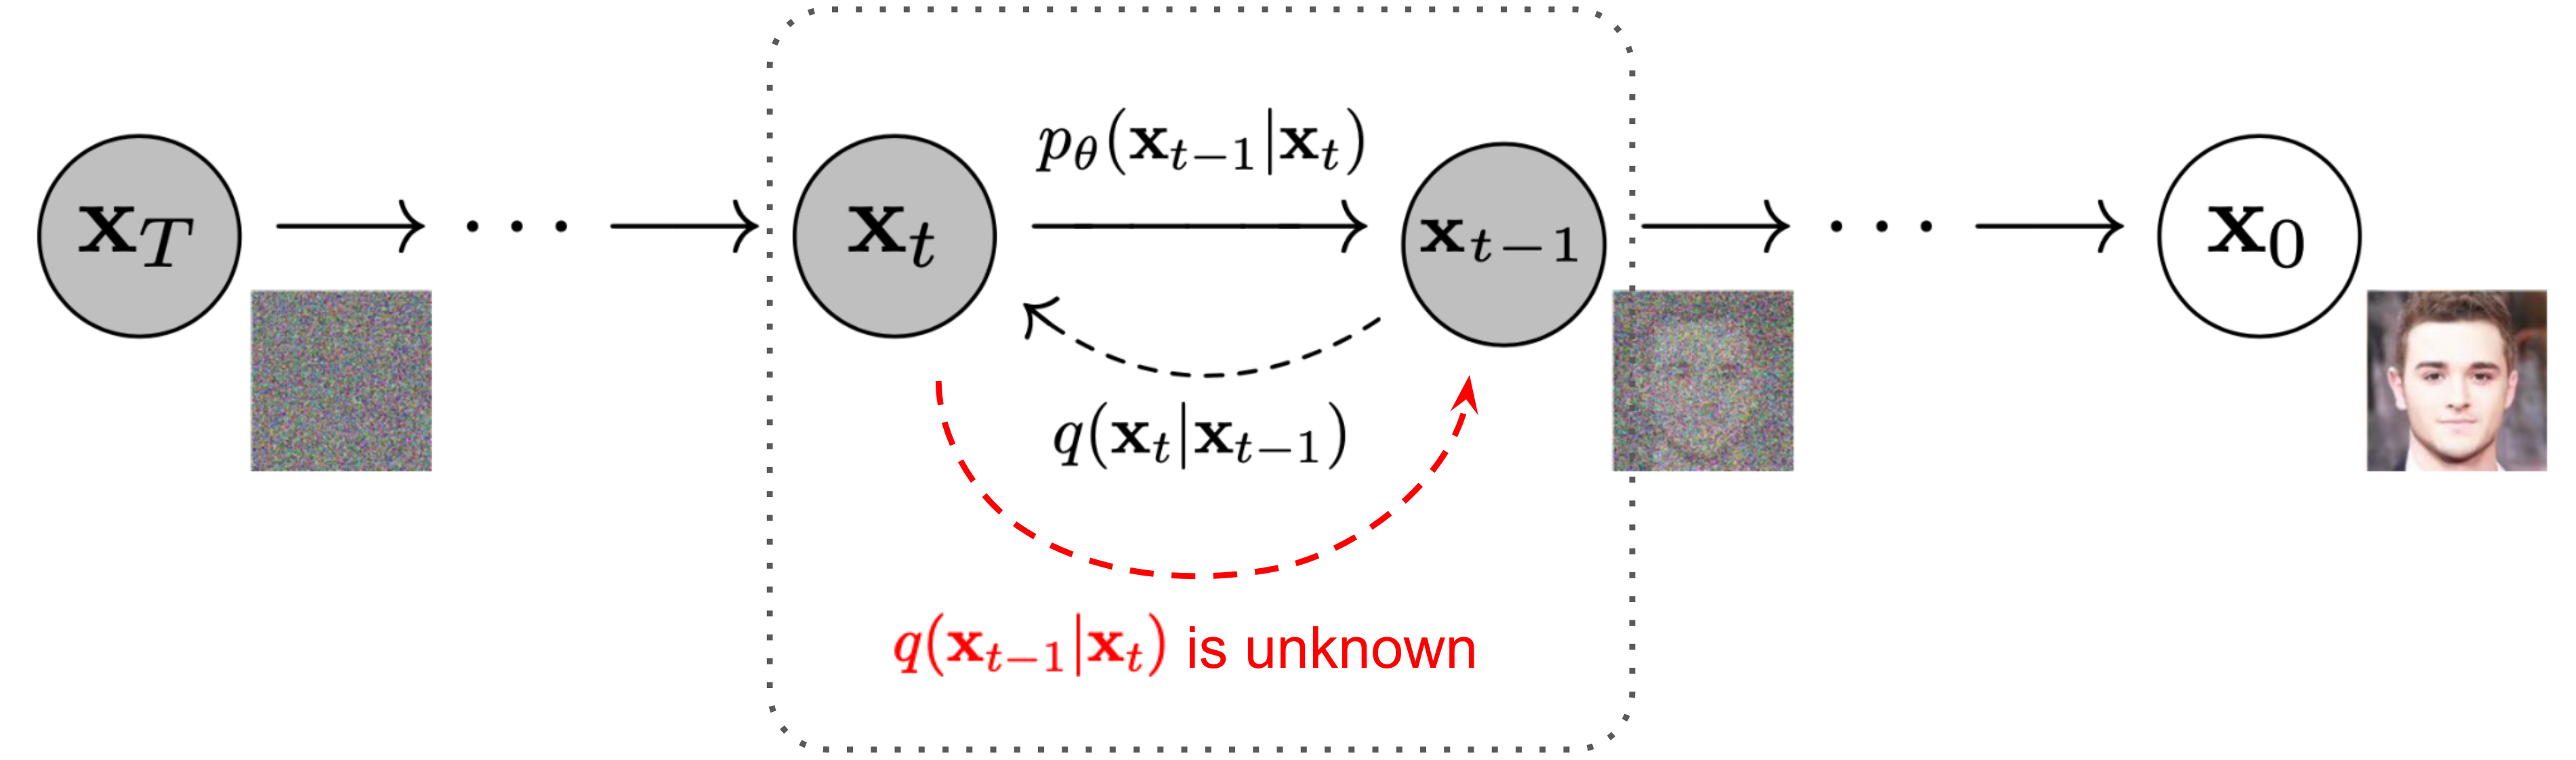
\includegraphics[width=0.8\linewidth]{figs/DDPM}
	\end{figure}
	\vspace{-0.3cm} 
	Let define the reverse process
	\vspace{-0.2cm}
	\[
		q(\bx_{t-1}|\bx_{t}) \approx p(\bx_{t - 1} | \bx_t, \btheta) = \cN \bigl(\bx_{t - 1} | \bmu_{\btheta}(\bx_t, t), \bsigma_{\btheta}^2(\bx_t, t)\bigr)
	\]
	\vspace{-0.7cm}
	\begin{minipage}{0.5\linewidth}
		\begin{block}{Forward process}
			\begin{enumerate}
				\item $\bx_0 = \bx \sim \pi(\bx)$;
				\item $\bx_t = \sqrt{1 - \beta} \cdot \bx_{t - 1} + \sqrt{\beta} \cdot \bepsilon$, where $\bepsilon \sim \cN(0, \bI)$, $t \geq 1$;
				\item $\bx_T \sim p_{\infty}(\bx) = \cN(0, \bI)$.
			\end{enumerate}
		\end{block}
	\end{minipage}%
	\begin{minipage}{0.5\linewidth}
		\begin{block}{Reverse process}
			\begin{enumerate}
				\item $\bx_T \sim p_{\infty}(\bx) = \cN(0, \bI)$;
				\item $\bx_{t - 1} = \bsigma_{\btheta}(\bx_t, t) \cdot \bepsilon + \bmu_{\btheta}(\bx_t, t)$;
				\item $\bx_0 = \bx \sim \pi(\bx)$;
			\end{enumerate}
		\end{block}
	\end{minipage}
	\textbf{Note:} The forward process does not have any learnable parameters!
	\myfootnotewithlink{https://lilianweng.github.io/posts/2021-07-11-diffusion-models/}{Weng L. What are Diffusion Models?, blog post, 2021}
\end{frame}
%=======
\section{Denoising diffusion probabilistic model (DDPM)}
%=======
\subsection{Objective of DDPM}
%=======
\begin{frame}{Gaussian diffusion model as VAE}
	\vspace{-0.2cm}
	\begin{figure}
		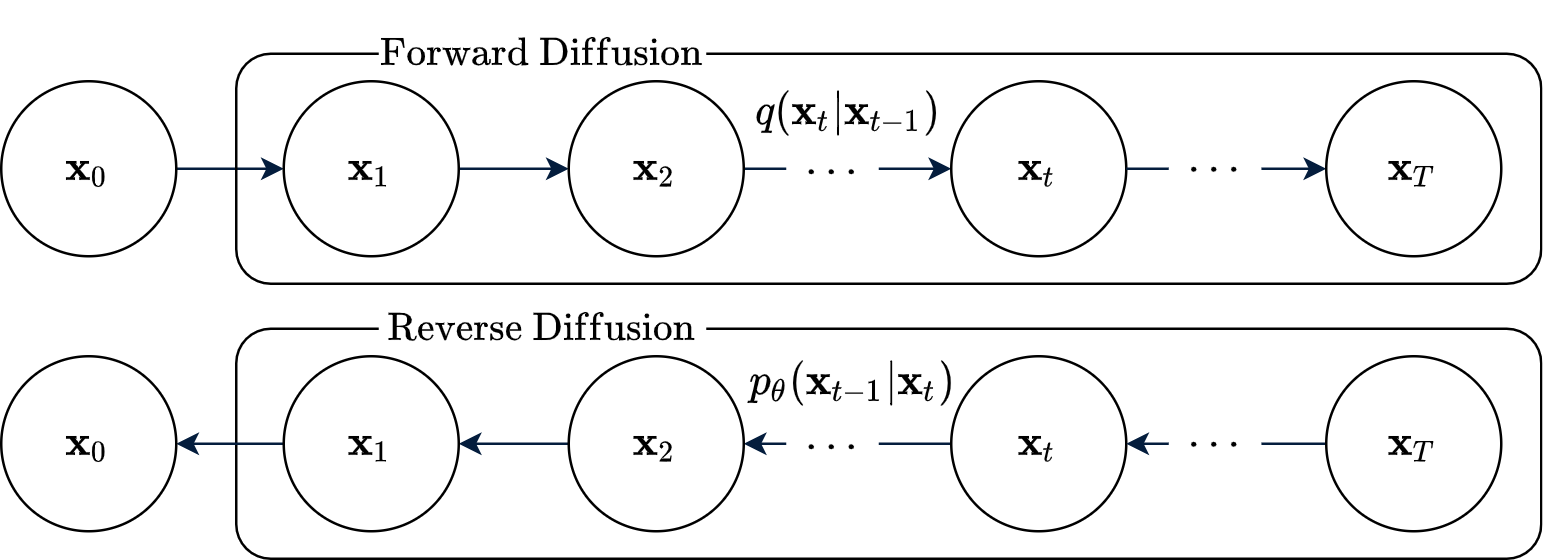
\includegraphics[width=0.65\linewidth]{figs/diffusion_pgm}
	\end{figure}
	\begin{itemize}
		\item Let treat $\bz = (\bx_1, \dots, \bx_T)$ as a latent variable (\textbf{note:} each $\bx_t$ has the same size).
		\item Variational posterior distribution (\textbf{note:} there is no learnable parameters)
		\vspace{-0.4cm}
		\[
			q(\bz | \bx) = q(\bx_1, \dots, \bx_T | \bx_0) = \prod_{t = 1}^T q(\bx_t | \bx_{t - 1}).
		\]
		\vspace{-0.5cm}
		\item Probabilistic model
		\vspace{-0.2cm}
		\[
			p(\bx, \bz | \btheta) = p(\bx | \bz, \btheta) p(\bz | \btheta)
		\]
		\item Generative distribution and prior
		\vspace{-0.3cm}
		\[
			p(\bx | \bz, \btheta) = p(\bx_0 | \bx_1, \btheta); \quad 
			p(\bz | \btheta) = \prod_{t=2}^T p(\bx_{t - 1} | \bx_t, \btheta)  \cdot p(\bx_T)
		\]
	\end{itemize}
	\myfootnotewithlink{https://ayandas.me/blog-tut/2021/12/04/diffusion-prob-models.html}{Das A. An introduction to Diffusion Probabilistic Models, blog post, 2021}
\end{frame}
%=======
\begin{frame}{Objective of DDPM}
	\begin{block}{ELBO}
		\vspace{-0.4cm}
		\[
			\log p(\bx | \btheta) \geq \bbE_{q({\color{teal}\bz} | \bx)} \log \frac{p(\bx, {\color{teal}\bz} | \btheta)}{q({\color{teal}\bz} | \bx)} = \cL(q, \btheta) \rightarrow \max_{q, \btheta}
		\]
		\vspace{-0.5cm}
	\end{block}
	\begin{block}{Derivation}
		\vspace{-0.5cm}
		{\small
		\begin{align*}
			\cL(q, \btheta) &= \bbE_{q({\color{teal}\bx_{1:T}} | \bx_0)} \log \frac{p(\bx_0, {\color{teal}\bx_{1:T}} | \btheta)}{q({\color{teal}\bx_{1:T}} | \bx_0)} \\
			& = \bbE_{q(\bx_{1:T} | \bx_0)} \log \frac{p(\bx_T) \prod_{t=1}^T p(\bx_{t-1} | \bx_t, \btheta) }{\prod_{t=1}^T q(\bx_t | \bx_{t-1})}  \\ 
			& = \bbE_{q(\bx_{1:T} | \bx_0)} \log \frac{p(\bx_T) p(\bx_0 | \bx_1, \btheta) \prod_{t=2}^T p(\bx_{t-1} | \bx_t, \btheta) }{q(\bx_1 | \bx_0)\prod_{t=2}^T {\color{teal}q(\bx_t | \bx_{t-1})}}  \\ 
			& = \bbE_{q(\bx_{1:T} | \bx_0)} \log \frac{p(\bx_T) p(\bx_0 | \bx_1, \btheta) \prod_{t=2}^T p(\bx_{t-1} | \bx_t, \btheta) }{q(\bx_1 | \bx_0)\prod_{t=2}^T q(\bx_t | \bx_{t-1}, {\color{olive}\bx_0})} 
		\end{align*}
		}
		\[
			q(\bx_{t-1}|\bx_{t}, {\color{olive}\bx_0}) = \frac{q(\bx_{t}|\bx_{t-1}, {\color{olive}\bx_0}) q(\bx_{t-1} | {\color{olive}\bx_0}) }{q(\bx_{t}| {\color{olive}\bx_0})} = \cN(\tilde{\bmu}_t(\bx_t, \bx_0), \tilde{\beta}_t \bI)
		\]
	\end{block}
	
	\myfootnotewithlink{https://arxiv.org/abs/2006.11239}{Ho J. Denoising Diffusion Probabilistic Models, 2020}
\end{frame}
%=======
\begin{frame}{Objective of DDPM}
	\begin{block}{Derivation (continued)}
		\vspace{-0.7cm}
		{\small
		\begin{multline*}
			\cL(q, \btheta) = \bbE_{q(\bx_{1:T} | \bx_0)} \log \frac{p(\bx_T) p(\bx_0 | \bx_1, \btheta) \prod_{t=2}^T p(\bx_{t-1} | \bx_t, \btheta) }{q(\bx_1 | \bx_0)\prod_{t=2}^T q(\bx_t | \bx_{t-1}, {\color{olive}\bx_0})}  = \\ 
			= \bbE_{q(\bx_{1:T} | \bx_0)} \log \frac{p(\bx_T) p(\bx_0 | \bx_1, \btheta) \prod_{t=2}^T p(\bx_{t-1} | \bx_t, \btheta) }{{\color{violet}q(\bx_1 | \bx_0)}\prod_{t=2}^T \frac{q(\bx_{t-1}|\bx_t, \bx_0) {\color{violet}q(\bx_{t} | \bx_0)}}{{\color{violet}q(\bx_{t-1}| \bx_0)}}}  = \\
			= \bbE_{q(\bx_{1:T} | \bx_0)} \log \frac{{\color{violet}p(\bx_T)} {\color{olive}p(\bx_0 | \bx_1, \btheta)} \prod_{t=2}^T p(\bx_{t-1} | \bx_t, \btheta) }{{\color{violet}q(\bx_T | \bx_0)}\prod_{t=2}^T q(\bx_{t-1}|\bx_t, \bx_0)}  = \\
			= \bbE_{{\color{teal}q(\bx_{1:T} | \bx_0)}} \biggl[ \log {\color{olive}p(\bx_0 | \bx_1, \btheta)} + \log {\color{violet}\frac{p(\bx_T)}{q(\bx_T | \bx_0)}} + \sum_{t=2}^T \log \left( \frac{p(\bx_{t-1} | \bx_t, \btheta)}{q(\bx_{t-1}|\bx_{t}, \bx_0)}\right) \biggr] = \\
			 = \bbE_{{\color{teal}q(\bx_1 | \bx_0)}} \log p(\bx_0 | \bx_1, \btheta) + \bbE_{{\color{teal}q(\bx_T | \bx_0)}} \log \frac{p(\bx_T)}{q(\bx_T | \bx_0)} + \\
			  + \sum_{t=2}^T \bbE_{{\color{teal}q(\bx_{t-1}, \bx_t | \bx_0)}} \log \left( \frac{p(\bx_{t-1} | \bx_t, \btheta)}{q(\bx_{t-1}|\bx_{t}, \bx_0)}\right) 
		\end{multline*}
		}
		\vspace{-0.3cm}
	\end{block}
	\myfootnotewithlink{https://arxiv.org/abs/2006.11239}{Ho J. Denoising Diffusion Probabilistic Models, 2020}
\end{frame}
%=======
\begin{frame}{Objective of DDPM}
		\vspace{-0.5cm}
		\begin{multline*}
			\cL(q, \btheta) = \bbE_{q(\bx_1 | \bx_0)} \log p(\bx_0 | \bx_1, \btheta) + \bbE_{q(\bx_T | \bx_0)} \log \frac{p(\bx_T)}{q(\bx_T | \bx_0)} + \\
			  + \sum_{t=2}^T \bbE_{q(\bx_{t-1}, \bx_t | \bx_0)} \log \left( \frac{p(\bx_{t-1} | \bx_t, \btheta)}{q(\bx_{t-1}|\bx_{t}, \bx_0)}\right) =
			  \\ =  {\color{olive}\bbE_{q(\bx_1 | \bx_0)} \log p(\bx_0 | \bx_1, \btheta)} - {\color{violet}KL\bigl(q(\bx_T | \bx_0) || p(\bx_T)\bigr)} - \\
			- \sum_{t=2}^T  \bbE_{q(\bx_t | \bx_0)} \underbrace{KL \bigl(q(\bx_{t-1} | \bx_t, \bx_0) || p(\bx_{t - 1} | \bx_t, \btheta )\bigr)}_{\cL_t}
		\end{multline*}
		\vspace{-0.5cm}
	\begin{itemize}
		\item {\color{olive}First term} is a decoder distribution
		\[
			\log p(\bx_0 | \bx_1, \btheta) = \log \cN \bigl(\bx_0 | \bmu_{\btheta}(\bx_1, t), \bsigma_{\btheta}^2(\bx_1, t)\bigr).
		\] 
		\item {\color{violet}Second term} is constant ($p(\bx_T)$ is a standard Normal, $q(\bx_T | \bx_0)$ is a non-parametrical Normal).
	\end{itemize}
	\myfootnotewithlink{https://arxiv.org/abs/2006.11239}{Ho J. Denoising Diffusion Probabilistic Models, 2020}
\end{frame}
%=======
\begin{frame}{Objective of DDPM}
	\vspace{-0.5cm}
	\begin{multline*}
		\cL(q, \btheta) =  {\color{olive}\bbE_{q(\bx_1 | \bx_0)} \log p(\bx_0 | \bx_1, \btheta)} - {\color{violet}KL\bigl(q(\bx_T | \bx_0) || p(\bx_T)\bigr)} - \\
		- \sum_{t=2}^T  \bbE_{q(\bx_t | \bx_0)} \underbrace{KL \bigl(q(\bx_{t-1} | \bx_t, \bx_0) || p(\bx_{t - 1} | \bx_t, \btheta )\bigr)}_{\cL_t}
	\end{multline*}
	$q(\bx_{t-1} | \bx_t, \bx_0)$ defines how to denoise a noisy image $\bx_t$ with access to what the final, completely denoised image $\bx_0$ should be.
	
	\begin{figure}
		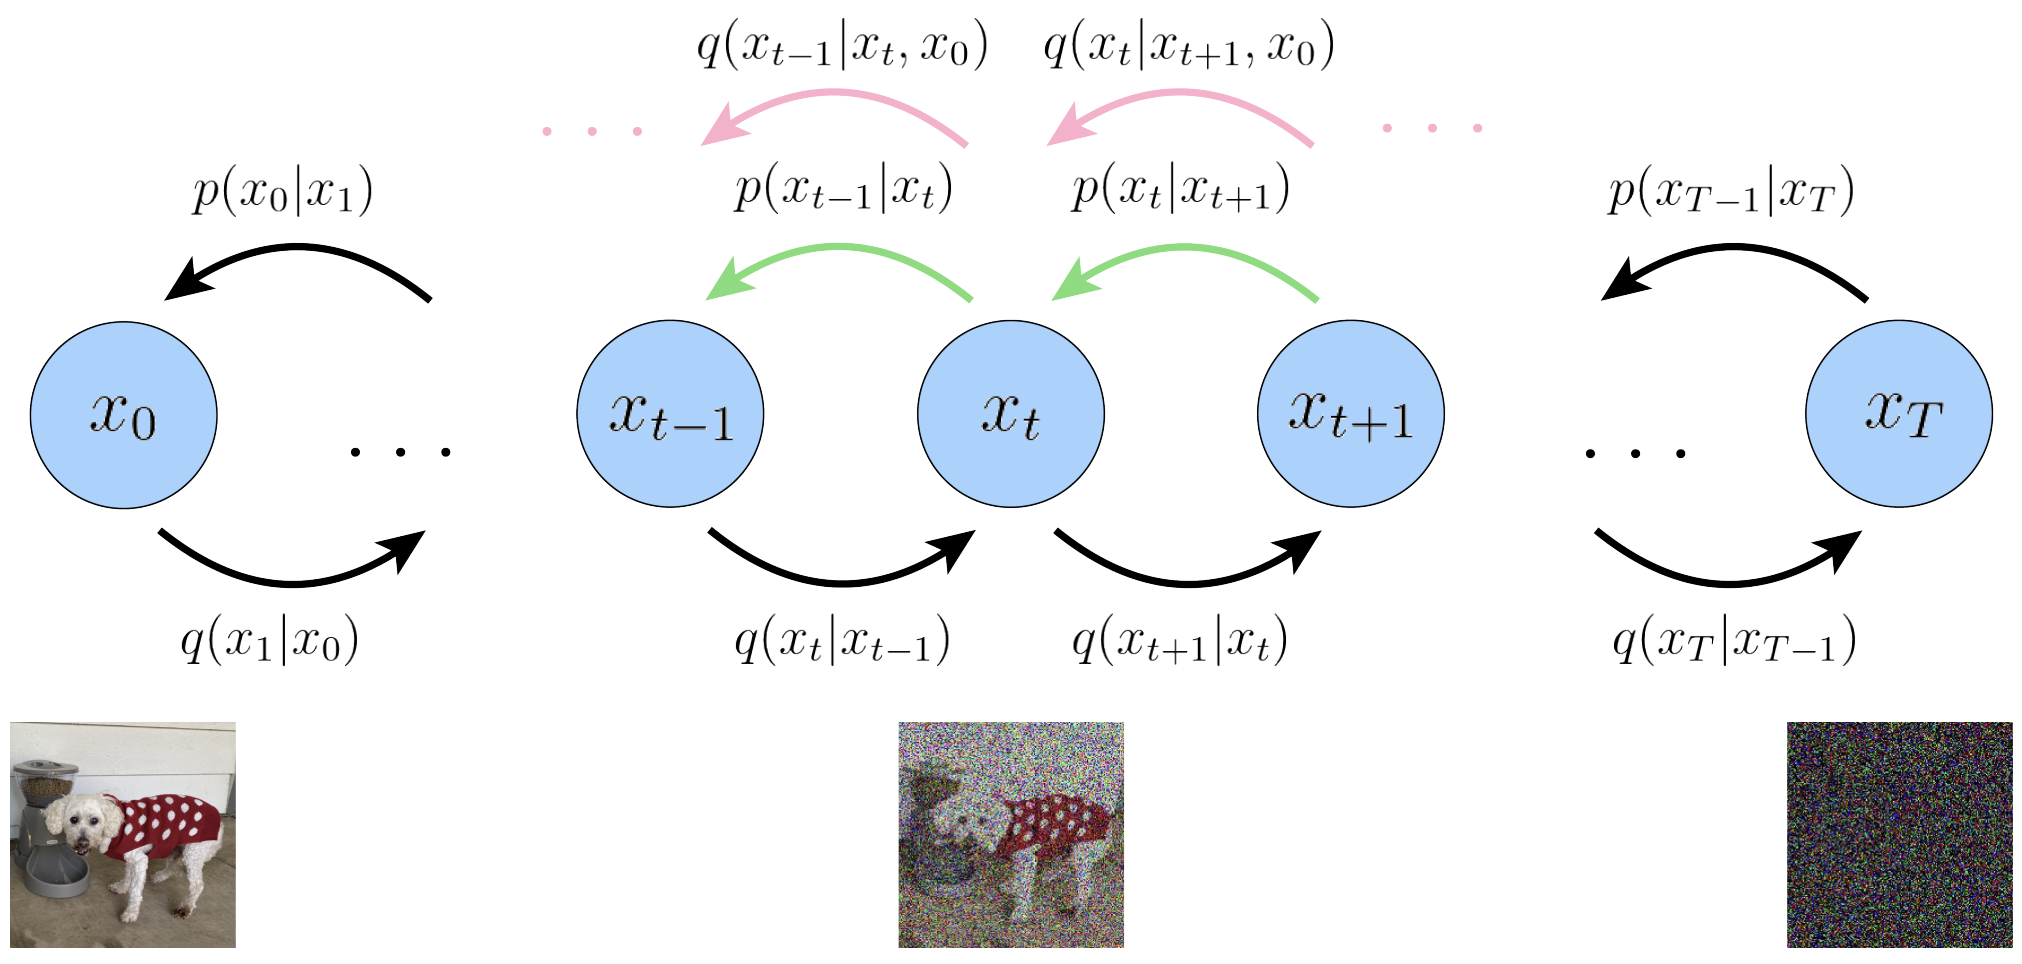
\includegraphics[width=0.85\linewidth]{figs/diffusion_objective}
	\end{figure}

	\myfootnotewithlink{https://arxiv.org/abs/2208.11970}{Luo C. Understanding Diffusion Models: A Unified Perspective, 2022}
\end{frame}
%=======
\subsection{Reparametrization of DDPM}
%=======
\begin{frame}{Reparametrization of DDPM}
	\[
		\cL_t =  KL \bigl(q(\bx_{t-1} | \bx_t, \bx_0) || p(\bx_{t - 1} | \bx_t, \btheta )\bigr)
	\]
	$\cL_t$ is a KL between two normal distributions:
	\begin{align*}
		q(\bx_{t-1} | \bx_t, \bx_0) &= \cN(\bx_{t-1} | \tilde{\bmu}_t(\bx_t, \bx_0), \tilde{\beta}_t \bI), \\
		p(\bx_{t - 1} | \bx_t, \btheta) &= \cN \bigl(\bx_{t - 1} | \bmu_{\btheta}(\bx_t, t), \bsigma_{\btheta}^2(\bx_t, t)\bigr)
	\end{align*}
	Here
	\begin{align*}
		\tilde{\bmu}_t(\bx_t, \bx_0) &= \frac{\sqrt{\alpha_t}(1 - \bar{\alpha}_{t-1})}{1 - \bar{\alpha}_t} \bx_t + \frac{\sqrt{\bar{\alpha}_{t-1}}(1 - \alpha_t)}{1 - \bar{\alpha}_t} \bx_0 \\
		\tilde{\beta}_t &= \frac{(1 - \alpha_t)(1 - \bar{\alpha}_{t-1})}{1 - \bar{\alpha}_t} = \text{const}
	\end{align*}
	Let assume
	\[
		\bsigma_{\btheta}^2(\bx_t, t) = \tilde{\beta}_t \bI \quad \Rightarrow \quad p(\bx_{t - 1} | \bx_t, \btheta) = \cN \bigl(\bx_{t - 1} | \bmu_{\btheta}(\bx_t, t), \tilde{\beta}_t \bI \bigr).
	\]
	\myfootnotewithlink{https://arxiv.org/abs/2006.11239}{Ho J. Denoising Diffusion Probabilistic Models, 2020}
\end{frame}
%=======
\begin{frame}{Reparametrization of DDPM}
	\vspace{-0.5cm}
	\begin{align*}
		q(\bx_{t-1} | \bx_t, \bx_0) &= \cN(\bx_{t-1} | \tilde{\bmu}_t(\bx_t, \bx_0), \tilde{\beta}_t \bI), \\
		p(\bx_{t - 1} | \bx_t, \btheta) &= \cN (\bx_{t - 1} | \bmu_{\btheta}(\bx_t, t), \tilde{\beta}_t \bI )
	\end{align*}
	Use KL formula between two normal distributions:
	\begin{align*}
		\cL_t &= KL\Bigl(\cN\bigl(\tilde{\bmu}_t(\bx_t, \bx_0), \tilde{\beta}_t \bI \bigr) || \cN\bigl(\bmu_{\btheta}(\bx_t, t), \tilde{\beta}_t \bI\bigr)\Bigr) \\ 
		&= \frac{1}{2\tilde{\beta}_t} \bigl\| \tilde{\bmu}_t(\bx_t, \bx_0) - \bmu_{\btheta}(\bx_t, t) \bigr\|^2 
	\end{align*}
	\[
		\bx_t = \sqrt{\bar{\alpha}_t} \bx_0 + \sqrt{1 - \bar{\alpha}_t} \bepsilon \quad \Rightarrow \quad {\color{olive} \bx_0} = \frac{\bx_t -  \sqrt{1 - \bar{\alpha}_t} \bepsilon}{\sqrt{\bar{\alpha}_t}}
	\]
	\begin{align*}
		\tilde{\bmu}_t(\bx_t, \bx_0) &= \frac{\sqrt{\alpha_t}(1 - \bar{\alpha}_{t-1})}{1 - \bar{\alpha}_t} \bx_t + \frac{\sqrt{\bar{\alpha}_{t-1}}(1 - \alpha_t)}{1 - \bar{\alpha}_t} {\color{olive} \bx_0} \\
		&= \frac{1}{\sqrt{\alpha_t}} \bx_t - \frac{1 - \alpha_t}{\sqrt{\alpha_t (1 - \bar{\alpha_t})}} \bepsilon
	\end{align*}
	\myfootnotewithlink{https://arxiv.org/abs/2006.11239}{Ho J. Denoising Diffusion Probabilistic Models, 2020}
	\end{frame}
%=======
\begin{frame}{Reparametrization of DDPM}
	\vspace{-0.3cm}
	\[
		\cL_t = {\color{olive}\frac{1}{2\tilde{\beta}_t}} \bigl\| \tilde{\bmu}_t(\bx_t, \bx_0) - \bmu_{\btheta}(\bx_t, t) \bigr\|^2
	\]
	\vspace{-0.3cm}
	\begin{block}{Reparametrization}
		\vspace{-0.7cm}
		\begin{align*}
			\tilde{\bmu}_t(\bx_t, \bx_0) &= \frac{1}{\sqrt{\alpha_t}} \bx_t - \frac{1 - \alpha_t}{\sqrt{\alpha_t (1 - \bar{\alpha_t})}} \bepsilon \\
			\bmu_{\btheta}(\bx_t, t) &= \frac{1}{\sqrt{\alpha_t}} \bx_t - {\color{teal}\frac{1 - \alpha_t}{\sqrt{\alpha_t (1 - \bar{\alpha_t})}}} \bepsilon_{\btheta}(\bx_t, t)
		\end{align*}
		\vspace{-0.7cm}
	\end{block}
		\vspace{-0.5cm}
		\begin{align*}
			\cL_t &= \frac{(1 - \alpha_t)^2}{2\tilde{\beta}_t \alpha_t (1 - \bar{\alpha_t})} \bigl\| \bepsilon - \bepsilon_{\btheta}({\color{violet}\bx_t}, t) \bigr\|^2 \\
			& =	\frac{{\color{teal}(1 - \alpha_t)^2}}{{\color{olive}2\tilde{\beta}_t} {\color{teal}\alpha_t (1 - \bar{\alpha_t})}} \Bigl\| \bepsilon - \bepsilon_{\btheta}\bigl( {\color{violet}\sqrt{\bar{\alpha}_t} \bx_0 + \sqrt{1 - \bar{\alpha}_t} \bepsilon}, t\bigr) \Bigr\|^2
		\end{align*}
		At each step of reverse diffusion process we try to predict the noise $\bepsilon$ that we used in forward process!
	\myfootnotewithlink{https://arxiv.org/abs/2006.11239}{Ho J. Denoising Diffusion Probabilistic Models, 2020}
	\end{frame}
%=======
\begin{frame}{Summary}
	\begin{itemize}
		\item Gaussian diffusion process is a Markov chain that injects special form of Gaussian noise to the samples.
		\vfill
		\item Reverse process allows to sample from the real distribution $\pi(\bx)$ using samples from noise.
		\vfill
		\item Diffusion model is a VAE model which reverts gaussian diffusion process using variational inference.
		\vfill
		\item ELBO of DDPM could be represented as a sum of KL terms.
		\vfill
		\item At each step DDPM predicts the noise that was used in forward diffusion process.		
	\end{itemize}
\end{frame}
\end{document} 